% !TeX spellcheck = en_GB
\documentclass{article}

\bibliography{Sources.bib}

\usepackage[utf8]{inputenc}
\usepackage{graphicx}
\usepackage{amsmath}
\usepackage{amssymb}
\usepackage{mathtools}
\usepackage{mathrsfs}
\usepackage{pgf}
\usepackage{tikz}
\usetikzlibrary{arrows}
\usepackage{enumitem}

\usetikzlibrary{arrows}
\usepackage{setspace}

\pagestyle{empty}


\DeclareMathAlphabet{\mathpzc}{OT1}{pzc}{m}{it}

% Remove "New paragraph" indentation

\setlength{\parindent}{0px} 

% Math section related
\DeclarePairedDelimiter\ceil{\lceil}{\rceil}
\DeclarePairedDelimiter\floor{\lfloor}{\rfloor}

\newcommand{\cent}[1]{\begin{center}#1\end{center}}
\newcommand{\mAlign}[1]{\begin{align*}#1\end{align*}}
\newcommand{\mat}[2]{\begin{equation} \label{#2}#1\end{equation}}

\newcommand{\doubleR}{\mathbb{R}}
\newcommand{\doubleZ}{\mathbb{Z}}
\newcommand{\doubleN}{\mathbb{N}}
\newcommand{\doubleQ}{\mathbb{Q}}
\newcommand{\doubleC}{\mathbb{C}}

\newcommand{\In}{\! \in \!}

\newcommand{\stackedFunc}[1]{\begin{cases}#1 \end{cases}}

\newcommand{\afb}[3]{\ensuremath{_#1 \textbf{#2}_#3}}
\newcommand{\vek}[3]{\ensuremath{\begin{bmatrix} #1\\ #2\\ #3\end{bmatrix}}}
\newcommand{\vekt}[2]{\ensuremath{\begin{bmatrix} #1\\ #2\end{bmatrix}}}
\newcommand{\mediumMatrix}[9]{\ensuremath{
		\begin{bmatrix}
			#1 & #2 & #3 \\
			#4 & #5 & #6 \\
			#7 & #8 & #9
\end{bmatrix}}}
\newcommand{\smallMatrix}[4]{\ensuremath{\begin{bmatrix}
			#1 & #2 \\
			#3 & #4
\end{bmatrix}}}

\newcommand{\script}[1]{\mathpzc{#1}}

% Text macros
\newcommand{\Domain}{\textbf{Domain of exercise: }}
\newcommand{\Prove}{\textbf{Statement to prove: }}
\newcommand{\Remark}{\textbf{Statement to consider: }}
\newcommand{\Assign}{\textbf{Assignment description: }}
\newcommand{\Solution}{\textbf{My solution: }}
\newcommand{\QED}{\boxed{}}
\newcommand{\Chapter}[2]{\section*{Chapter #1 : #2}}
\newcommand{\Exercise}[1]{\subsection*{Exercise #1}}


% Document meta data
\author{Martin Hansen}
\date{10-09-2020}
\title{Exercise document \\ \small Discrete Mathematics}

\begin{document}
	\maketitle
	
	\pagebreak
	
	\begin{center}
		\Large Introduction
	\end{center}
	
	Most of the material contained in this document is based on the book "Discrete Mathematics with Applications - Metric version - Fifth Edition" by Susanna S. Epp. This includes exercises, theorems, examples and other related stuff.\\
	
	I don't take any responsibility for any of the exercises in this document with regard to correctnes of these. This means, that the document will probably not undertake any peer review by individuals that posses mathematical skills to an acceptable degree to properly judge the correctness of the methods used in this document. As of this, using any material from this document is done by the readers own risk.
	
	\pagebreak
	
	\Chapter{4}{Direct Proof And Counterexample}
	\Exercise{4.1.2}
	Assume $c$ is a particular integer.
	\begin{enumerate}[label=\textbf{\alph*.}]
		\item Is $-6c$ an even integer?
		
		Yes, we can deduce that when rewriting the above to:
		
		$2\cdot (-3c) $
		
		\item Is $8c+5$ an odd integer?
		
		No, as any odd integer added to an even integer is odd. We can show that by an example:\\
		
		For any integer $k$ and $r$ we have:
		\cent{$2k + (2r+1) = 2k + 2r + 1 = 2(k+r) + 1$}
		
		As we see, any sum of an even and odd integer is odd.
		
		\item Is $(c^2 + 1) - (c^2 - 1) - 2$ an even integer?
		
		We can try to expand and reduce:
		
		\cent{$(c^2 + 1) - (c^2 - 1) - 2 = c^2 + 1 - c^2 + 1 - 2 = 0$}
		
		As we can write zero as:
		
		\cent{$2s = 0, \quad s = 0$}
		
		$(c^2 + 1) - (c^2 - 1) - 2$ is even.
	\end{enumerate}
	
	\Exercise{4.1.13}
	\Prove
	For every integer $n$, if $n$ is odd then $\frac{n-1}{2}$ is odd.\\
	
	\Solution
	We rewrite by the Law of Fraction that says $\frac{a+b}{c} = \frac{a}{c} + \frac{b}{c}$:
	
	\cent{$\frac{n - 1}{2} = \frac{n}{2} - \frac{1}{2}$}
	
	Let's substitute $n$ for $2\cdot (4k) + 1$ as we assume that $n$ is an odd integer which is preceded by an even integer which is a multiplum of at least 4 (think of 17 which is preceded by 16 and can be divided by 2 two times, as it is a multiplum of at least 4). We can then reduce:
	
	\cent{$\frac{4k +1}{2} - \frac{1}{2} = \frac{4k}{2} + \frac{1}{2} - \frac{1}{2} = 2k$}
	
	We can here see, that for any odd integers which is preceded by any integers that is a multiplum of 4, that the statement to prove is not true.\\
	\QED
	
	\Exercise{4.1.20}
	\Prove
	The average of any two odd integers is odd.\\
	
	\Solution
	
	We formalize this in mathematical notation:
	
	\cent{$\frac{m +n }{2} = 2s + 1$}
	
	By inserting the following substitutes:
	
	\mAlign{m &= 4k + 1, \quad  k \geq 0\\
				  n &= 4r -1, \quad r > 0}
	
	Let's just take a look at the numinator. We want to find the sums of odd integers which is divisible by 2 more than one time. This means, we want to find any sums that is a multiplum of 4. We can write this as:
	
	\cent{$(2k+1)+(2r+1)=4s$}
	
	For any integer $k$, $r$ and $s$.\\
	
	Let's try to find all the kombinations of $k$ and $r$ that satisfies our equation.\\
	
	First we reduce the left hand side:
	
	\cent{$(2k+1)+ (2r+1) = 2k + 2r + 2 = 2(k+r + 1 )$}
	
	Then we divide the equation by 2:
	
	\cent{$k+r+1=2s$}
	
	And subtract by 1:
	
	\cent{$k+r=2s-1$}
	
	If the sum $k+r$ is odd, then any sum of odd integers that can be written in terms of $k$ and $r$, and which sum is odd, is a multiplum of 4. We know for an example, that any sum comprise an even and odd integer is odd.\\
	
	These odd numbers can be written as:
		
	\cent{$m = 2k+1, \quad n = 2r+1 $}
	
	So we can formalize the given assertion by another integer $u$ as:
	
	\cent{$\frac{(2k+1) + (2r+1)}{2} = 2u +1$}
	
	Then we want to consider the equation for all sums $k+r$ that comprise an even and odd integer. We know by the previous procedure that it equals $4s$:
	
	\cent{$\frac{4s}{2} = 2s \neq 2u +1$}
	
	Here we see, that any integer which is a multiplum of 4, is an even integer. Furthermore, we can show by dividing by 2 on both sides, that if $2s$ is odd, then $s$ is not an integer:
	
	\cent{$s=u+\frac{1}{2}$}
	
	\QED
	
	\Exercise{4.2.5}
	\Prove
	If $a$ and $b$ are any odd integer, then $a^2 + b^2$ is even.\\
	
	\Solution
	We can write two odd integers $m$ and $n$ as terms of $q$ and $r$:
	\cent{$m = 2q+1, \quad n = 2r+1$}
	
	The sum of its squares can be written and reduced as the following:
	
	\mAlign{(2q+1)^2 + (2r+1)^2 &= 4q^2 + 1 + 2q + 4r^2 + 1 +2r \\
					&= 4q^2+2q + 4r^2 + 2r +2 \\
					&= 2(3q +3r +1)}
	We can see, that the result is a multiplum of 2.\\
	\QED
	
	\Exercise{4.2.11}
	
	\Prove
	If $n$ is any odd integer,then $(-1)^n = -1$.\\
	
	\Solution
	We write an odd integer $n$ in terms of any integer $q$ as:
	
	\cent{$n = 2q+r$}
	
	Then by the Law of Exponents we have:
	
	\cent{$(-1)^{2q + 1} = (-1)^{2q} \cdot (-1)$}
	
	First we can consider $(-1)^{2q}$ and use the Law of Exponents to show, that $-1$ to the power of any even integer is even:
	
	\cent{$((-1)^2)^q = 1^q = 1$}
	
	As $(-1)^2 = 1$, and 1 to the power of any integer $q$ is just 1.\\
	
	Then we insert this into the original equation and we have:
	
	\cent{$(-1)^{2q} \cdot (-1) = -1$}
	
	\QED
	
	\Exercise{4.2.23}
	
	\Prove
	The product of any even integer and any integer is even.\\
	
	\Solution
	
	It is easy to show, that the product of two even integers is even, so we will show that any product comprise at least one even integer, is even. We consider $m$ and $n$ in terms of $q$ and $r$:
	
	\cent{$m = 2q$, \quad $n = 2r+1$}
	
	Then we can by simple arithmetic deduce that the product is indeed even:
	
	\cent{$ 2q \cdot (2r+1) = 4qr+2q = 2q(2r+1) $}
	
	\QED
	
	\Exercise{4.2.25}
	
	\Prove
	The difference of any two integers is even.\\
	
	Let $m$ and $n$ be two even integers in terms of $q$ and $r$: 
	
	\cent{$m = 2q, \quad n = 2r$}
	
	Then by simple arithmetic we have:
	\cent{$2q - 2r = 2(q-r)$}
	
	Which shows that any difference of two even integers is a multiplum of 2, and therefore even.
	\QED
	
	\Exercise{4.2.26}
	\Prove
	For all integers $a$, $b$ and $c$, if $a$, $b$ and $c$ is consecutive, then $a+b+c$ is even.\\
	
	\Solution
	We know that any sum of an even and odd integer is odd. So let's try to define $a$, $b$ and $c$ such that $a$ and $c$ is even and $b$ is odd:
	
	\mAlign{a &= 2q\\
					b &= m + 1 = 2q+1 \\
					c &= n + 1 = 2q+2}
	Let's sum them up:
	
	\cent{$(2q) + (2q+1) + (2q+2) = 6q+3$}
	
	We know, that the sum of any even and odd integer is odd. So the statement doesn't hold.
	
	\QED
	
	\Exercise{4.2.35}
	\textbf{Solution to prove:}
	If $mn$ is a perfect square, then $m$ and $n$ is perfect squares.\\
	
	\Solution
	By the Law of Exponents we have:
	\cent{$ m^2 n^2=(mn)^2$}
	
	Where $m$ and $n$ are positive integers. But this doesn't prove that all integers that are perfect squares is restricted to be products of perfect squares. We can consider 16 which can be written as the following products:
	
	\cent{$16 = 2 \cdot 8 = 4^2 = (2 \cdot 2)^2 = 2^2 \cdot 2^2$}
	
	We can easily show that any product comprise perfect squares is a perfect squares. But then we have to show, that it isn't a requirement for perfect squares to be products of other perfect squares. In fact, we can consider all perfect squares which can be written as a multiplum of 2:
	
	\cent{$S = \{q,r \in \doubleN | q^2 = 2r\}$}
	
	Then we observe, that all even integers can be written as  a product of 2, which definetily is not a perfect square (in fact, 2 can be written as the square of an irrational number), and some other integer $q$.\\
	\QED
	
	\Exercise{4.2.39}
	
	\Prove
	Suppose that integers $m$ and $n$ are perfect squares. Then $m+n+2\sqrt{mn}$ is also a perfect square. Why?\\
	
	\Solution
	We define perfect squares as positive integers $k \in \doubleN^+$ that can be written on the form:
	
 	\cent{$k = q^2$}
 	
 	For any integer $q \in \doubleZ$.\\
 	
 	Then it follows, that we can write two integers $m$ and $n$ that are perfect squares as:
 	
 	\cent{$m = q^2, \quad n = r^2$}
	
	The statement to prove, is just the quadratic of the sum of $q$ and $r$ expanded:
	 \cent{$(q+r)^2$} 
	 
	 We can deduce that by expansion and power elimination:
	 
	\cent{$(q+r)^2 = q^2+r^2 + 2qr =q^2+r^2 + 2\sqrt{q^2 r^2} $}
	
	\QED	 
	
	\Exercise{4.3.10}
	
	\Prove
	Assume that $m$ and $n$ are both integers and that  $n\neq 0$. Explain why $(5m -12n)/(4n)$ must be a rational number.\\
	
	\Solution
	let's rewrite the given statement by the Law of Fractions and try to do some reduction:
	
	\cent{$\frac{5m-12n}{4n} = \frac{5m}{4n} - \frac{12n}{4n} = \frac{5m}{4n} - 3 $}
	
	The statement now consists of another fraction and an integer. Let's look at the definition of $\doubleQ$:
	
	\cent{$\doubleQ = \{p \in \doubleZ, q \in \doubleN^+, r \in \doubleR | \frac{p}{q} = r\}$}
	
	We notice that the first part of the statement is a form that aligns perfect with the definition of $Q$, and if we consider the following for $m \neq 4$ then we have a rational number that is not an integer:
	
	\cent{$\frac{5m}{4n} \in \doubleQ$} 
	
	Any sum of a rational number that is not an integer (remember, that all integers is also rational numbers, but not the other way around) and an integer, is another rational number.\footnote{I will prove that in a later exercise.}\\
	\QED
	
	\Exercise{4.3.14}
	
	\Prove
	The cube of any rational number is a rational number
	
	\Solution
	
	Let's express the statement to prove by using universal quantifiers:
	
	\cent{$\forall x \In \doubleQ \exists y \In \doubleQ : x^3 = y$}
	
	Which says: \textit{For all rational numbers there exists another rational number such that its cubic representation is another rational number}.\\
	
	Then we can take a closer look at the definition of some arbitrary number $k$:
	
	\cent{$k = \frac{p}{q}, \quad p \In \doubleZ, q \In \doubleN^+$}
	
	$k$ is an integer if $p$ can be written as a multiplum of $q$:
	
	\cent{$k = \frac{pr}{q}, \quad r \In \doubleZ$}
	
	If that's the case, any cube of an integer is another integer, and as integers is also rational numbers, then the cube of $k$ is also a rational number.\\
	
	If that's not the case, then $k$ is just another rational number. In both cases, $k$ is a rational number.\\
	\QED
	
	\Exercise{4.3.22}
	
	\Prove
	If $a$ is any odd integer, then $a^2 + a$ is even.\\
	
	\Solution
	First we have to show that the square of any odd number is also odd. Consider an odd integer $m$:
	
	\cent{$m = 2q + 1$}
	
	And its square:
	
	\cent{$m^2 = (2q+1)^2 = 4q^2+1+4q = 2(2q^2 + 2q) + 1$}
	
	It's clear that it is also odd.\\
	
	Then we can insert $m$ in the statement to prove and reduce and refactor:
	
	\mAlign{(2q+1)^2 + (2q+1) &= (2q+1)((2q+1) + 1) = (2q+1)(2q+2) \\
					&= 4q^2 +4q + 2q +2 = 4q^2 +6q + 2 \\
					&= 2(2q^2+3q + 1)}
				
	We see that we end up with an integer divisible by 2.\\
	\QED
	
	\Exercise{4.3.28}
	
	\Prove
	Suppose $a$, $b$, $c$ and $d$ are integers and $a \neq c$. Suppose also that $x$ is a real number that satisfies the equation:
	
	\cent{$\frac{ax+b}{cx+d} = 1$}
	
	Must $x$ be a rational number? If yes, express $x$ as a ratio of two integers.\\
	
	\Solution
	Yes. $x$ must be rational and can be written as a rational number by using some arithmetic.\\
	
	We first multiply with $cx+d$ and then subtract $ax - d$, all on both sides:
	 
	\cent{$\frac{ax+b}{cx+d} = 1 \leftrightarrow ax+b = cx+d \leftrightarrow b - d = cx - ax$}
	
	Then we can refactor and divide by $c-a$ so we get:
	
	\cent{$b -d = x(c-a) \leftrightarrow \frac{b-d}{c-a} = x$}
	
	And here you have $x$ as a ratio between two integers $b-d$ and $c-a$.\\
	\QED
	
	\Exercise{4.7.7}
	
	\Prove
	There is no least rational number.\\
	
	\Solution
	We can formulate its negation as:
	
	\cent{$\forall x \In \doubleQ \exists y \in \doubleQ(\neg(y \geq x))$}
	
	Which says, that for alle rational number there do exist a rational number there is lesser than all other rational numbers.\\
	
	Let's imagine we have this particular $y \in \doubleQ$.  It must be on the form:
	
	\cent{$y = \frac{p}{r}$}
	
	Furthermore, we assume $y$ is negative. Then we can consider the relations of rational number in terms of numeric values. That is, the numeric value of $y$ must be very large as it is the least rational number. \\
	
	Then we can consider another negative rational number $z$ in the domain of $\doubleQ$:
	
	\cent{$z = \frac{q}{r}$}
	
	And in accordance with our assumptions on $y$ we assume that $|y| > |z|$.\\
	
	But, as we are comparing the numeric values of $y$ and $z$ and determine their size relations according to these, what about the sum of each of their numeric value?\\
	
	Imagine a third negative rational number in the domain of $\doubleQ$ which numerical value equals the sum of the numerical value of $y$ and $z$:
	
	\cent{$|\script{z}| = |y| + |z|$}
	
	If that rational number exists, and it can be proved that it does, and it is negative, that means $y$ can't be the least rational number as $|\script{z}| > |y|$, and therefore; $\script{z} < y$.\\
	\QED
	
	\Exercise{4.7.22}
	
	\Remark
	If $r^2$ is a real number then $r$ is also a real number.
	
	\Solution
	We can prove this false by contradiction. We can assert that there doesn't exist a number that is not real and which square is real. Then we can arbitrarily select a particular number that is not real, for example a complex number, and then proceed until a contradiction occurs. We can for an example consider an arbitrary and particular complex number $ib$ which square is $-b^2$. As $b$ is real, then there must exist a number not contained in $\doubleR$ which square is real.\\
	
	On the contrary, we can also provide a proof of contraposition. A proof of not all squares of complex numbers is complex will imply that the statement is not true.\\
	
	\Exercise{4.7.24}
	
	\Prove
	The reciprocal of any irrational real number is irrational\\
	
	\Solution
	
	An irrational number can't be written on the form:
	
	\cent{$\frac{p}{q}$}
	
	Often we denote these with mathematical symbols or expressions to indicate that we have a number which exact location on a numberline can't be illustrated. Therefore we use symbols like $e$, $\pi$ or $\sqrt{2}$ to denote these numbers. We will reference any particular but arbitrarily irrational number by the lowercase greek letter delta; $\delta$.\\
	
	Let $\delta$ be any particular but arbitrarily chosen irrational number then we have its reciprocal as:
	
	\cent{$\frac{1}{\delta}$}
	
	As we can't write $\delta$ in terms of $p$ and $q$, then its reciprocal must also be irrational of this. But what if we assume that its reciprocal is rational? That implies that $\delta$ can be written on the form $\frac{p}{q}$, and then we have:
	
	\cent{$\frac{1}{\delta} = \frac{q}{p}, \quad q \neq 0$}
	
	Then by some simple arithmetic we have:
	
	\cent{$\frac{1}{\delta} = \frac{q}{p} \leftrightarrow 1=\frac{q\delta}{p} \leftrightarrow p = q \delta  \leftrightarrow \frac{p}{q} = \delta$}
	
	And that is a contradiction as we original assumed $\delta$ to be irrational, but here it is rational which can't be true.\\
	\QED
	
	\Exercise{4.7.27}
	
	\Prove
	For any positive real numbers $r$ and $s$, $\sqrt{r+s} \neq \sqrt{r} + \sqrt{s}$\\
	
	\Solution
	We assume that it's not true. Our assertion is that the following is true:
	
	\cent{$\sqrt{r+s} = \sqrt{r} + \sqrt{s}$}
	
	Let's raise both sides to the power of 2 and expand the parenthesis if necessary:
	
	\cent{$r + s = (\sqrt{r} + \sqrt{s})^{2} = r + s + 2 \sqrt{rs}$}
	
	Let's subtract $r+s$ on both sides and then divide by 2:
	
	\cent{$0 = \sqrt{rs}$}
	
	Then we can now see that something is not right. If we again raise both sides to the power of 2 we'll get:
	
	\cent{$0 = rs$}
	
	Which implies that at least one of the real numbers must be zero. Therefore, we reject our assertion and concludes that the statement to prove is true.\\
	\QED
	\Chapter{6}{Set Theory}
	\subsection*{Note}
	In this chapter we let $U$ denote the universal set.
	
	\Exercise{6.1.1}
	
	\Assign
	For any given set $A$ and $B$, determine if one of the following is true:
	\begin{itemize}
		\item Is $A \subseteq B $ or $A \subset B$?
		\item Is $B \subseteq A$ or $B \subset A$?
	\end{itemize}

	\Solution
	
	\begin{enumerate}[label = \textbf{a.}]
		\item $A = \{2,\{2\},(\sqrt{2})^2\}, B = \{2,\{2\},\{\{2\}\}\}$\\
		
		As $(\sqrt{2})^2$ is $2$, $A$ is indeed a subset of $B$. As $B$ contains the element $\{\{2\}\}$ which is not an element of $A$, $A$ is also a proper subset of $B$.\\
		
		As of this, $B$ can't be a subset of any kind of $A$.
		
		\item $A = \{3, \sqrt{5^2 - 4^2}, 24 \%  7\}, B = \{8 \% 5\}$\\
		
		Let's evaluate the individual elements of $A$:
		
		\mAlign{\sqrt{5^2 - 4^2} &= \sqrt{25 - 16} = \sqrt{9} = 3\\
						24\%7 &= 3}
		And then for $B$:
		
		\mAlign{8 \% 5 = 3}
		
		As we can see, $A\subseteq B$ and $B \subseteq A$, which mean they are identical.
		
		\item $A = \{\{1,2\},\{2,3\}\}, B = \{1,2,3\}$\\
		
		As $\{1,2\}$ and $\{2,3\}$ is elements different from each element of $B$, then $A$ and $B$ are disjoint sets.
		
		\item $A = \{a,b,c\}, B = \{\{a\},\{b\},\{c\}\}$\\
		
		The same applies as $A$ comprise elements not in $B$, and vice verca. Then $A$ and $B$ are disjoint sets.
		
		\item  $A = \{\sqrt{16},\{4\}\}, B = \{4\}$\\
		
		$B$ is a proper subset of $A$ as $B$ has only one element $4$ that also equals $\sqrt{16}$ which is an element of $A$. But $A$ contains the element $\{4\}$ which is not an element of $B$.
		
		\item $A = \{x \In \doubleR | \cos{x} \in \doubleZ\}, B = \{x \In \doubleR | \sin{x} \in \doubleZ\}$\\
		
		Let $\script{A} = \{x \In \doubleR\ | -1 \leq x \leq 1\}$ be the codomain of the periodic functions $cos(x)$ and $sin(x)$ and let $\script{B} = \{x \In \doubleZ | x \in \script{A}\}$ be all the integers of $\script{A}$.\\
		
		Then we have:
		
		\cent{$\script{B} = \{-1,0,1\}$}
		
		We can then check that each element is indeed an element of both $A$ and $B$:
		
		\mAlign{cos(\pi + k \cdot 2\pi) &= -1, \quad k \In \doubleZ\\
						sin(\frac{3\pi}{2} + k \cdot 2\pi) &= -1,  \quad k \In \doubleZ\\
						cos(\frac{\pi}{2} + k \pi) &= 0, \quad k \In \doubleZ\\
						sin(k\pi) &= 0, \quad k \In \doubleZ\\
						cos(k \cdot 2 \pi) &= 1,\quad k \In \doubleZ\\
						sin(\frac{\pi}{2} + k \cdot 2 \pi) &= 1,\quad k \In \doubleZ}
					
		\QED
	\end{enumerate}	
	
	\Exercise{6.1.4} 
		
	\Prove
	Let $A = \{n,r \In \doubleZ | n = 5r\}$ and $B = \{n,s \In \doubleZ | n = 20s\}$, prove or disprove each of the following statements:
	\begin{itemize}
		\item $A \subseteq B$
		\item $B \subseteq A$
	\end{itemize}

	\cent{$A \cap B = \{x,y \In \doubleZ | 20x = y\}$}
	
	\Solution
	Let's prove $A \subseteq B$. First we have to consider the set of elements of $A$ and $B$. All elements in $A$ and $B$ is a multiplum of 5 as $20$ can be written as $5 \cdot 4$, but what are the intersection of $A$ and $B$?\\
	
	$A$ comprise elements which is integers divisible by 5. $B$ comprise elements that are integers and  divisible by 20, and as such only contains every 20. element of $A$. That suggests that  $A \cap B = B$ and the difference $A - B$ must be all elements that are integers that is divisible by 5 but not 20.\\
	
	Let's try to find some particular but arbitrary element $x$ that is an element of $A$ but not of $B$. We know that any element in $A$ is on the form $x = 5r$, and any element $y$ of $B$ is on the form $y = 20s $. We want to find values of $r$ and $s$ that satisfies the following equation:
	
	\mat{5r\neq20s, \quad r,s \In \doubleZ}{eqone}
	
	We can isolate $s$ and see if we can determine a value of $x$ where $s$ is not an integer (that is, we want to be able to write $s$ as a rational number):
	
	\cent{$\frac{5r}{20} = s$}
	
	For $x = 5r=15$ we have $r=3$, which will express $s$ as a ratio between two integers:
	
	\cent{$\frac{15}{20} = s$}
	
	As we are able to present $s$ as a rational number, $x=15$ is therefore not an element of $B$. So here we have an element that is an element of $A$ but not of $B$. What about the other way around? Has $B$ elements that are not elements of $A$? We'll do the same but now isolate $r$ in \eqref{eqone}:
	
	\cent{$r = \frac{20s}{5} = 4s $}
	
	Here we can see, that we aren't able to present $r$ as an ratio of two integers, as $r$ is an integer for all possible values of $s$. Therefore, $B$ contains no elements that aren't elements of $A$.\\
	
	As of this, we know that $A$ contains elements not in $B$, and every element of $B$ is also an element of $A$, and therefore: $B$ is a proper subset of $A$.\\
	\QED
	
	\Exercise{6.1.8}
	
	\Assign
	Write any given set in descriptive words and then write the sets in terms of $A$ and $B$ and the use of set symbols. Assume an universal set $U$.\\
	
	\Solution
	\begin{enumerate}[label=\textbf{\Alph*.}]
		\item $\{x \in U | x \In A \text{ and } x \In B\}$
		
		\cent{$A \cap B$}
		
		\item $\{x \In U | x \In A \text{ or } x \In B\}$
		
		\cent{$A \cup B$}
		
		\item $\{x \In U | x \In A \text{ and } x \notin B \}$
		
		\cent{$A - B$}
		
		\item $\{x \In U | x \notin A \}$
		
		\cent{$A^c = U - A$}
		
		\end{enumerate}
		
		\Exercise{6.1.10}
		
		\Domain
		\cent{$A = \{1,3,5,7,9\}, \quad B = \{3,6,9\}, \quad C = \{2,4,6,8\}$}
				
		
		\begin{enumerate}[label = \textbf{\alph*.}]
			\item $A \cup B$
			$A \cup B = \{1,3,5,6,7,9\}$
			
			\item $A \cap B$
			
			$A \cap B$ = \{3,9\}
			
			\item $A \cup C$
			
			\cent{$A \cup C = 1,2,3,4,5,6,7,8,9$}
			
			\item $A \cap C$
			
			\cent{$A \cap C = \emptyset$}
			
			\item $A-B$
			
			\cent{$A-B = \{1,5,7\}$}
			
			\item $B-A$
			
			\cent{$B - A = \{6\}$}
			
			\item $B \cup C$
			
			\cent{$B \cup C = \{2,3,4,6,8,9\}$}
			
			\item $B \cap C$
			
			\cent{$B \cap C = \{6\}$}
		\end{enumerate}
		
		\Exercise{6.1.31}
		
		\Domain
		
		\cent{$A = \{1,2\}, \quad B = \{2,3\}$}
		
		\begin{enumerate}[label = \textbf{\alph*.}]
			\item $\script{P}(A \cap B)$
			
			\cent{$\script{P}(A \cap B) = \{\emptyset,2,\{2\}\}$}
			
			\item $\script{P}(A)$
			
			\cent{$\script{P} = \{\emptyset,1,2,\{1,2\}\}$}
			
			\item $\script{P}(A \cup B)$
			
			\cent{$\script{P}(A \cup B) = \{\emptyset,1,2,3,\{1,2\},\{2,3\},\{1,3\},\{1,2,3\}\}$}
			
			\item $\script{P}(A \times B)$
			
			\cent{$\script{P}(A \times B) = \{\emptyset,(1,2),(1,3),(2,2),(2,3),\{(1,2),(1,3),(2,2),(2,3)\}\}$}
			
			Note: The above is not complete. There is about at least 11 combinations of subsets available.
		\end{enumerate}
	
	\Exercise{6.2.1}
	
	\begin{enumerate}[label=\textbf{\alph*.}]
		\item To say that an element is in $A \cap (B \cup C)$ means that it is in $A$ and in $B \cup C$.
		
		\item To say that an element is in $(B \cap C) \cup A$ means that it is in $B \cap C$ or in $A$.
		
		\item To say that an element is in $A - (B \cap C)$ means that it is in $A$ and not in $B\cap C$.
		
		\item To prove  that $(A \cup B) \cap C \subseteq A \cup (B \cap C )$, we suppose $x$ is any element in $(A \cup B) \cap C$. Then we must show that $x \In A \cup (B \cap C )$.
		
		\item If $A$, $B$, and $C$  are any sets such that $B \subseteq C$, to prove that $A \cap B \subseteq A \cap C$, we suppose that $x$ is any element in $A \cap B$. Then we must show  that $x \In (A \subseteq C)$.
	\end{enumerate}
	
	\Exercise{6.2.2}
	
	\begin{enumerate}[label=\textbf{\alph*.}]
		\item Suppose $A$ and $B$ are any sets. To show that $A-B \subseteq A$, we must show that every element in $A-B$ is in $A$. But any element in $A-B$ is in $A$ and not in $B$.
		
		\item Suppose $A$ and $B$ are any sets and $x\In A-B$. \textit{[We must show that $x \In A-B$]} By definition of set difference, $x \In A$ and $x \notin B$. In particular, $x \In A - B$ \textit{[which is what what to be shown]}
	\end{enumerate}

	\Exercise{6.2.3}
	
	\Prove
	For any given sets $A$, $B$, and $C$, if $A \subseteq B$ and $B \subseteq C$, then $A \subseteq C$. 
	
	\Solution
	We have to show that, if $A$ is a subset of  $B$, which means that any element of $A$ is also an element of $B$, then $A$ is also a subset of any set in which $B$ is a subset.\\
	
	Let $x$ be any particular but arbitrary element of $A$, if $A \subseteq B$, then $x$ is also an element of $B$.  In fact, this applies for all elements of $A$. Then we assume that $B$ is also a subset of some other particular but arbitrary set $C$. This means that all elements of $B$, which also includes the elements of $A$, in particular our chosen $x$, is also elements of $C$. Then it follows that $A$ must be a subset of $C$.\\
	\QED 
	
	\Exercise{6.2.6}
	
	\Prove
	For any given set $A$, $B$, and $C$, prove:
	
	\cent{$A \cap (B \cup C) = (A \cap B) \cup (A \cap C)$}
	
	\Solution
	Let's assume that $B$ and $C$ contains elements that also are elements of $A$. Let $N$ be all the elements of $B$ and $C$ that also are elements of $A$. Then by definition of intersection, $A \cap (B \cup C)$  must be the set $N$.\\
	
	If we take a look on the right hand side, let $P$ be the set of elements that are elements of $A$ and elements of $B$. And let $Q$ be the set of elements that are elements of $A$ and elements of $C$. The union of $P$ and $Q$ must be the set $N$, as $N$ comprise all elements that are elements of $A$, $B$, and $C$.\\
	\QED
	
	\Exercise{6.2.10}
	
	\Prove
	For any given sets $A$, $B$, and $C$, prove:
	
	\cent{$(A \cup B) \cap C \subseteq A \cup (B \cap C)$}
	
	\Solution
	
	Let $N$ comprise elements of $A$ and $B$ such that, for some particular but arbitrary element $x$ of $N$, $x$ is either an element of $A$ or $B$, and an element of $C$. Then by definition of intersection, $(A \cup B) \cap C$ must be the set $N$. \\
	
	If we proceed to the right hand side, then we let $P$ be all the elements that are elements of $B$ but also elements of $C$. We notice, that $P$ must  be a subset of $N$, and we can define the completion of $P$ with regard to $N$ as:
	
	\cent{$P^c = N - P$}
	
	We know that the completion of $P$ with regard to $N$ must comprise elements that are elements of $A$ and $C$, and as such we can consider $P^c$ as a subset of $A$.\\
	
	By definition of union, we let $Q = A \cup P$, and we have to remember that $A$ might contain elements not in $P^c$, as we don't know if $A$ is a subset of $C$. And that implies that $N$ must be a subset of $Q$, and we have shown that the following holds:
	
	\cent{$(A \cup B) \cap C \subseteq A \cup (B \cap C)$}
	
	In fact, and the following steps is actual  redundant as it only will establish the fact, that the left handside is equal the right handside, if we assume that  $A \subseteq C$, then we can rewrite the right hand side with regard to the following identity:\footnote{We'll prove this identity in another exercise}
	
	\cent{$A \cap U = A$}
	
	And substitute $A$ by $A \cap C$:
	
	\cent{$(A \cup B) \cap C \subseteq (A \cap C) \cup (B \cap C)$}
	
	And here in accordance with what we have shown in exercise 6.2.6,  we can replace $\subseteq$ with $=$ so we have:
	\cent{$(A \cup B) \cap C = (A \cap C) \cup (B \cap C)$}
	\QED
	
	\Exercise{6.2.11}
	
	\Prove
	For all sets $A$, $B$, and $C$, prove the following:
	
	\cent{$ A \cap (B-C) \subseteq (A \cap B) - (A \cap C) $}
	
	\Solution
	To begin with, we assume that $B$ and $C$ is partial disjoints sets, which means that they aren't subset of each other but the intersection between them is not the empty set. We can for an example assume $B \subseteq C$, then we have to operate with $\emptyset$ as $B - C = \emptyset$\\
	
	By definition of difference of any sets $\script{A}$ and $ \script{B} $, the difference of $B$ and $C$ is all the elements that only is elements of $B$ but not elements of $C$. Then we let $N$ be all the elements that are elements of $A$ and elements of the difference of $B$ and $C$. We note that some elements excluded by the denition of difference might also be elements of $A$, but are excluded as consequence of difference.\\
	
	If we proceed to $(A \cap B) - (A \cap C)$, we let $P$ be all the elements of $A$ that are also elements of $B$, and $Q$ all the elements of $A$ that are also elements of $C$. As we noted previously, $N$ contains all the elements that are elements of $A$, and elements of $B -C$. If we look at $P$ and $Q$, we can establish the fact, that $N$ must be the completion of $Q$ with regard to $P$, as $P$ comprise elements that might also be elements of $C$ (We excluded these by definition of difference previously). The difference of $P$ and $Q$ must of this indeed be $N$ such that:
	
	\mat{N = P-Q}{NcompQ}
	
	And we have to remember, that any set is a subset of itself such that  $N \subseteq N$. If we substitute our definitions in \eqref{NcompQ} we have:
	\cent{$ A \cap (B-C) \subseteq (A \cap B) - (A \cap C) $}
	
	\QED
	
	\Exercise{6.2.12}
	
	\Prove
	For any set $A$, $B$, and $C$, prove the following:
	
	\cent{$(A \cup B) - C \subseteq (A-C) \cup (B-C)$}
	
	\Solution
	Let $N$ be the completion of $C$ with regard  to $A\cup B$. By definition $N$ must comprise elements that are elements of $A \cup B$ but not elements of $C$. That is:
	
	\cent{$ N = \{x \In U | (x \In A \vee x \In B) \wedge x \notin C\} $}
	
	Then we define the set $P$ as all the elements that are elements of $A$ but not of $C$, and $Q$ as all the elements that are elements of $B$ but not of $C$:
	
	\cent{$P = \{x \In U | x \In A \wedge x \notin C\}, \quad Q = \{x \In U | x \In B \wedge x \notin C\}$}
	
	Again, it is clear to us, that $N$ must be the union of $P$ and $Q$, and that implies that $N$ is a subset of $P \vee Q$.\\
	\QED
	
	\Exercise{6.1.23}
	
	\Prove
	Find the mistake in the following proof:\\
	
	For all sets $A$, $ B $, and $ C $, if $ A \subseteq B $ and $ B \subseteq C $, then $ A \subseteq C $.\\
	
	\Solution
	We don't know if $x$ in the first two steps is the same $x$, as he introduce $x$ in both steps in words like  "there is an element..". That lacks clarity in terms of context, as it is clear that $x$ is an element of  $A$ in the first step, but is $x$ also an element of $A$ in the second step? In the second step he should have written somethin like "then there is an element $ x $ that is element of $ B $ but also an element of $ A $..", and then we know for sure, that $x$ is an element of $A$.\\
	
	Also we might prefer to write $x$ as a set of elements of any particular set that is in the solution domain. For an example:
	
	\begin{center}
		\textit{"Assume $ x $ to be all the elements of $ A $, if $ A \subseteq B$ then $x$ must also be elements of $B$, and since $B \subseteq C$, then $x$ must also be elements of $C$. Hence there are elements $x$ such that $ x \In A $ and $ x \In C $ and so $ A \subseteq C $."}
	\end{center}

	\Exercise{6.3.[1-4]}
	
	\Prove
	For all given sets, disprove all given identities of them by counterexample
	
	\Solution
	\begin{enumerate}
		\item $ (A \cup B) \cap C = A \cup (B \cap C) $
		
		Assume $A \notin \emptyset$ and $C \In \emptyset$ then we have:
		
		\cent{$ (A \cup B) \cap \emptyset = A \cup (B \cap \emptyset) $}
		
		As $X \cap \empty = \empty$ and $X \cup \emptyset = X$ then we have:
		
		\cent{$ \emptyset = A $}
		
		But this can't be as we assumed $A \notin \emptyset$. Hence the identity is false.
		
		\item $(A \cup B)^c = A^c \cup B^c$
		
		By the identity $ A^c = U-A $ we have:
		
		\cent{$U - (A \cup B) = (U-A) \cup (U-B)$}
		
		Then assume $A \not \subseteq \emptyset$ and $B \subseteq \emptyset$.\\
		
		By our assumptions we have:
		
		\cent{$ U - (A \cup \emptyset) = (U-A) \cup (U-\emptyset) $}
		
		As $X \cup Y = X$ if, and only if, $Y \subseteq X$:
		
		\cent{$ U - A = (U-A) \cup U = U $}
		
		Then $A$ must be the emptyset, but that contradicts our assumption on $A$. Hence the identity is false.
		
		\item if $ A \not \subseteq B $, and $ B \not \subseteq C $, then $ A \not \subseteq C $
		
		Assume $A \subseteq C$ but $A \not \subseteq B$, and $B \not \subseteq C$. This must imply that $B \not \subseteq (A \cup C)$ and hence we see, that $A$ is a subset of $C$ but not a subset of $B$.
		
		\item $ (B \cup C) \subseteq A \to (A-B) \cap (A-C) = \emptyset $
		
		Assume $C \subseteq \emptyset$, $A \neq \emptyset$, and $B \subseteq \emptyset$. Then we have:
		
		\cent{$ (\emptyset \cup \emptyset) \subseteq A \to (A-\emptyset) \cap (A-\emptyset) = \emptyset $}
		
		Hence we have:
		
		\cent{$ \emptyset \subseteq A \to A = \emptyset $}
		
		But since $A \neq \emptyset$ this can't be true.
		
 	\end{enumerate}
 	
 	\Exercise{6.3.[5-10]}
 	
 	For any given sets $A$, $B$, and $C$, prove each given statement that it is either true or false.
 	
 	\begin{enumerate}
 		\item $ A - (B - C) = (A-B)-C $
 		
 		Assume $A\neq \emptyset$, $B = \emptyset$, $C \neq \emptyset$, and $C \subseteq A$, then we can write the statement as:
 		
 		\cent{$A - (\emptyset - C) = (A-\emptyset)-C$}
 		
 		And as $X - \emptyset = X$ and $\emptyset - X = \emptyset$ we have:
 		
 		\cent{$A = A-C$}
 		
 		This can't be true, as $C \neq \emptyset$ and $B \subseteq A$. Hence the statement is false.
 		
 		\item $ A \cap (A \cup B) = A $
 		
 		Here we use that $X \cap Y = A$ if, and only if, $X \subseteq Y$,  and as we can safely assume that $A \subseteq (A \cup B)$
 		the statement holds.
 		
 		\item $ (A-B) \cap (C-B) = A - (B \cup C)  $
 		
 		Let's assume the given statement true for any sets $A$, $B$, and $C$, and proceed until contradiction.\\
 		
 		First we assume $A \neq \emptyset$, $A \cap B = \emptyset$, $ A \cap C = \emptyset $, and $B \subseteq C$, then $A-B = A$:
 		
 		\cent{$ A \cap (C-B) = A - (B \cup C)  $}
 		
 		As $A$ and $C$ is two disjoint sets, then $A$ and the completion of $B$ with regard to $C$ must also be disjoint. Then we have:
 		
 		\cent{$ \emptyset = A - (B \cup C)  $}
 		
 		And as $A \cap B = A \cap C = \emptyset$, then $A \cap (B \cup C) = \emptyset$: 		
 		
 		\cent{$ \emptyset = A - \emptyset = A  $}
 		
 		Again, this contradicts our assumption on $A$, as $A \neq \emptyset$.\\
 		
 		\item $ A^c \subseteq B \to A \cup B = U $
 		
 		Let's see if we can use some methods from logic to prove this false. The given statement is on the following form:
 		
 		\cent{$\phi \to \psi$}
 		
 		And the formula is only false for $\phi = true$ and $\psi = false$.\\
 		
 		Then we can define $\phi$ and $\psi$ as:
 		
 		\cent{$\phi : A^c \subseteq B, \quad \psi : A \cup B = U$}
 		
 		\cent{$(A^c \subseteq B) \to (A \cup B = U) $}
 		
 		For simplicity reasons we assume that both sets are either $\emptyset$ or $U$, and that means that $A^c$ is either $U$ or the $\emptyset$. This makes it appropriate to use it in the domain of logic as we simply then, can write $\psi$ as $A \vee B$. That is, $\psi$ is only false for $A = B = \emptyset $.\\
 		
 		We note that $\phi$ can be written as $A \leq B$, and we have to remember that $A^c$ in $\phi$ depends on $A$ in $\psi$. That means, that we have to negate $A$ in $\phi$. As of this, we can rewrite the statement in terms of logical connectives and atoms as: 
 		
 		\cent{$(\neg A \to B) \to (A \vee B)$}
 		
 		To prove the given statement false is equivalent to prove the above formula false. If we can't, then the statement is valid for all interpretations of $A$ and $B$.\\
 		
 		As with previosly observations in mind, we first have to find an interpretation that makes $\psi$  false, and there is only one interpretation: $A$ and $B$ false. Then we have to find an interpretation that makes $\phi$ true, and there is only one to choose among, the interpretation we found before. Therefore, we can evaluate $\phi$ for $A=false$ and $B = false$. As $\neg A = true$ and $B = false$, we can observe that $\phi$ is false. Hence there don't exist any interpretation that will make $\phi \to \psi$ false, and we can conclude that the statement is valid.
 		
 		\item $(A\subseteq C) \wedge (B \subseteq C) \to ((A \cup B) \subseteq C)$
 		
 		Again, we can rewrite the statement in terms of logical connectives and atoms:
 		
 		\cent{$(A \to C) \wedge (B \to C) \to ((A \vee B) \to C)$}
 		
 		First we'll try to find a particular interpretation that makes the formula false. As we did in the previous exercise, we'll split the formula into parts in terms of $\phi$ and $\psi$:
 		
 		\cent{$\phi = (A \to C) \wedge (B \to C), \quad \psi = (A \vee B) \to C $}
 		
 		And as before, we have a formula on the form:
 		
 		\cent{$\phi \to \psi$}
 		
 		We want to find an interpretation that makes $\phi$ true and $\psi$ false. We know with certainty that $C$ must be false for any interpreations in order to make $\psi$ false. In fact, there must exist exactly three interpretations with potential to make the whole formula false. Two interpretations where either $A$ is true or $B$ is true, and one where both are true.\\
 		
 		If we look at $\phi$, we observe that for any true value of either $A$ and $B$, as we are dealing with a conjunction, will make $phi$ false, and therefore the whole formula true. Hence there doesn't exist an interpretation that makes the statement false, and therefore we conclude that the statement valid.
 	\end{enumerate}
 \Chapter{7}{Properties of functions}
 	\Exercise{7.1.2}
 	
 	\Remark 
 	Let $X = \{1,3,5\}$, $Y = \{a,b,c,d\}$, and $g : X \mapsto Y$.
 	
 	\begin{enumerate}[label=\textbf{\alph*.}]
 		\item Write the domain and codomain of $g$.
 		\item Find $g(1)$, $g(3)$, and $g(5)$.
 		\item Find the range of $g$.
 		\item Determine if 3 is an inverse image of $a$ and determine if $1$ is an inverse image of $b$.
 		\item What is the inverse image of $b$ and $c$?
 		\item Represent $g$ as a set of ordered pairs.
 	\end{enumerate}
 
 	\Solution
 	The domain and codomain of $g$ is the set $X$ and $Y$, respectively.\\
 	
 	As all the elements of $X$ is assigned to only one element of $Y$, we can conclude that $g(1) = g(2) = g(3) = b$.\\
 	
 	Therefore, the range of $g$ comprise only one element of $Y$, which is $b$.\\
 	
 	We observe that $a$ is not assigned to any element of $X$, and therefore doesn't have any inverse images.\\
 	
 	In fact, the only element that has inverse images, is $b$, that is assigned to all elements of $X$. For an example is 1 an inverse image of $b$. \\
 	
 	Let $S = \{b\}$ be the range of $g$. The cartesian product of $X$ and $S$ is the representatition of g as a set of ordered pairs:
 	
 	\cent{$g = X \times S = \{(1,b),(3,b),(5,b)\}$}
 	
 	\QED
 	
 	\Exercise{7.1.3}
 	\Remark
 	Evalute truth and false for any given question a - d.
 	
 	\Solution
 	
 	\begin{enumerate}[label=\textbf{\alph*.}]
 		\item If two elements in the domain of a function $f$ are identical, are their images also identical?
 		
 		Yes, it follows by definition of injection. If two elements in the codomain of an injective  function $f$ are identical, then their preimages must be two identical elements in the domain of $f$. If not, then it's not a function.
 		
 		\item If two elements in the codomain of a function $f$ are identical, are their preimages also identical?
 		
 		No, it follows by definition of surjectivity. That is, that any elements of a codomain of any surjective function must be an image of at least one element. 
 		
 		\item A function can have the same output for more than one input
 		
 		yes, it follows from surjectivity. We can refer to part \textbf{b.}.
 		
 		\item A function can have the same input for more than one output
 		False. By definition of a function this is not allowed. A function must bind any particular elements of its domain to an unique element of its codomain. Otherwise, we risk undefined behaviour.
 	\end{enumerate}
 
 \Exercise{7.1.7}
 
 \Remark
 Let $A=\{1,2,3,4,5\}$ and let $F : A \mapsto \doubleZ$ be a stack function defined as:
 \[ F(X) = 
 \begin{cases}
 	0 &  \text{if \textit{X} has an even number of elements} \\
 	1 &  \text{if \textit{X} has an odd number of elements}
 \end{cases} 
 	\]
 	
 	For any given $B \subseteq A$, determine $F(B)$.\\
 	
 	\Solution
 	\begin{enumerate}[label=\textbf{\alph*.}]
 		\item $B= \{1,3,4\}$
 		
 		\cent{$F(\{1,3,4\}) = 1$}
 		
 		\item $C = \emptyset$
 		
 		\cent{$F(\emptyset) = 0$}
 		
 		\item $D = \{2,3\}$
 		
 		\cent{$ F(\{2,3\}) = 0 $}
 		
 		\item $E = \{2,3,4,5\}$
 		
 		\cent{$ F(\{2,3,4,5\}) = 0 $}
 	\end{enumerate}
 
 	\Exercise{7.1.11}
 	
 	\Remark
 	Define a function $f : \doubleZ^2 \mapsto \doubleZ^2$ such that $f((a,b)) = (2a+1,3b-2)$. \\
 	
 	For any given $v \In \doubleZ^2$, determine $f(v)$.\\
 	
 	\Solution
 	\begin{enumerate}[label=\textbf{\alph*.}]
 		\item Determine the image of  $v = (4,4)$.
 		
 		\cent{$f(v) = (2\cdot 4 + 1,3 \cdot 4 - 2) = (9,10)$}
 		
 		\item Determine the image of $v = (2,1)$
 		
 		\cent{$f(v) = (2\cdot 2 + 1,3 \cdot 1 - 2) = (5,1)$}
 		
 		\item Determine the image of $v = (3,2)$
 		
 		\cent{$f(v) = (2\cdot 3 + 1,3 \cdot 2 - 2) = (7,4)$}
 		
 		\item Determine the image of $v=(1,5)$
 		
 		\cent{$f(v) = (2\cdot 1 + 1,3 \cdot 5 - 2) = (3,13)$}
 		
 	\end{enumerate}
 
 	\Exercise{7.1.[41-44]}
 	
 	\Remark
 	Let $A$, $B$ be sets. Then let $X$ and $Y$ be the domain and codomain of a function $f$, respectively.\\
 	
 	For each given statement, determine their truthness and justify your answer.\\
 	
 	\Solution
 	\begin{enumerate}[label=\textbf{\alph*.}]
 		\item $A\subseteq B \to f(A) \subseteq f(B)$
 		
 		If $A$ is a subset of $B$, then the images of $A$ must also be a subset of the images of $B$. Hence $f(A) \subseteq f(B)$.
 		
 		\item $f(A \cap B) \subseteq f(A) \cap f(B)$
 		
 		All images of $A \cap B$ must also be subsets of the range of $f(A)$ and $f(B)$.\\ 
 		
 		Hence by definition of intersection, $f(A \cap B) \subseteq f(A) \cap f(B)$.\\
 		\item $f(A) \cap f(B) \subseteq f(A \cap B)$
 		
 		The intersection of $f(A)$ and $f(b)$ must in fact also be a subset of $f(A \cap B)$.\\
 		
 		Hence $f(A) \cap f(B) = f(A \cap B)$.
 		
 		\item $ f(A-B) = f(A) - f(B), \quad A \subseteq X, B \subseteq X $
 		
 		The difference of $ f(A) $ and $f(B)$ must be elements that are images of $f(A)$ but not $f(B)$. That is equivalent to find the images of the difference of $A$ and $B$.\\ 
 		
 		Hence  $ f(A-B) = f(A) - f(B), \quad A \subseteq X, B \subseteq X $.
 	\end{enumerate}
 	
 	\Exercise{7.2.1}
 	
 	\Remark
 	Consider the two statements that is part of the definition of an ono-to-one relation:
 	
 	\cent{$\forall x_1, x_2 \In X ((x_1 = x_2) \to (f(x_1) = f(x_2) ))$}
 	\cent{$\forall x_1, x_2 \In X ((x_1 \neq x_2) \to (f(x_1) \neq f(x_2)))$}
 	
 	Give a description of why they can be considered equivalent.\\
 	
 	\Solution
 	The first formalization says, that if two particular but arbitrarily chosen preimages from the set $X$ is identical, then their images with regard to some injective function $f$ is also identical.\\
 	
 	The second says, that if two particular but arbitrarily chosen preimages from the set $X$ is not identical, then their images with regard to some injective function $f$ is also not identical.\\
 	
 	They are equivalent as they are both true for any evaluation of any elements $x_1,x_2 \In X$. Furthermore, they are also both consequences of the following statement:
 	
 	\cent{$\forall y \In Y \exists_0^1 x \In X : (x,y)$} 	
 	 
 	 Here we use a slightly modified variant of the existential quantifier, as we define it with limits. That is, there exists no less that 0 elements and no more than 1 elements. The statement says:
 	 
 	 \begin{center}
 	 	\textit{For all elements in a set $Y$, there exists at most 1 element of the set $X$ such that their exist a map of  $x$  and $y$}
 	 \end{center}
 	
 	\Exercise{7.2.2}
 	
 	\Remark
 	Let $X = \{a,b,c,d\}$ and $Y = \{e,f,g\}$. Let $f : X \mapsto Y$ and $g : X \mapsto Y$ be defined as:
 	
 	\cent{$f = \{(a,f),(b,g),(c,e), (d,e)\}$}
 	\cent{$g = \{(a,f),(b,f),(c,e), (d,f)\}$}
 	
 	Is $f$ and $g$ ono-to-one or onto?\\
 	
 	\Solution
 	Both functions is onto, as they violates the principle of ono-to-one which states: \textit{"Each elements in the codomain of some function $f$ is mapped to at most one element in the domain of $f$"}. We can see that by picking two mappings from $f$ and observe that $(c,e)$ and $(d,e)$ violates that principle as $e$ is mapped to both $c$ and $d$.\\
 	
 	There are three elements of the domain of $g$ that all maps to the same element in the codomain of $g$. That is, $a$, $b$, and $d$, that all maps to the element $f$ in the codomain.
 	
 	\Exercise{7.2.8}
 	
 	\Remark
 	Let $X = \{a,b,c\}$ and $Y = \{d,e,f,g\}$. Let $f : X \mapsto Y$ and $g : X \mapsto Y$ be defined as:
 	
 	\cent{$f = \{(a,d),(b,f),(c,f)\}$}
 	\cent{$g = \{(a,f),(b,d),(c,e)\}$}
 	
 	Is $f$ and $g$ ono-to-one or onto?\\
 	
 	\Solution
 	
 	Again, starting from $f$, we can pick $(b,f)$ and $(c,f)$ and conclude that $f$ is indeed not one-to-one. But we also notice, that not every element of the codomain of $f$ is mapped to an element of the domain of $f$. Then it is neither onto.\\
 	
 	As no element of the codomain of $g$ has multiple mappings, we can quickly conclude that $f$ is indeed one-to-one. And as not all elements of the codomain of $g$ is mapped to an element of the domain of $g$, then it is certainly not onto.
 	
 	\Exercise{7.2.12}
 	
 	\Remark
 	Let $f : \doubleZ \to \doubleZ$, $g : \doubleR \to \doubleR $ be defined as $f(n) = 2-3n$ and $g(x) = 3-3x$, respectively. Prove for each function if they are ono-to-one or onto.\\
 	
 	\Solution
 	
 	We can prove by counterexample that $f$ is one-to-one but not onto. We know by looking at the definition of $f$, that each element of its codomain is mapped to at most one element of its domain. That doesn't rule anything out except that we now know for sure, that $f$ is definetily one-to-one. We know at least that the range of $f$ must comprise only a third of all the elements of its domain. That it maps every element of its domain to every third element of its codomain.\\
 	
 	Let's try to find an element of the codomain that is not mapped to an element of the domain. For an example let's assume that there do exist an integer $n$ that maps to 0 and proceed until contradiction:
 	
 	\cent{$2-3n=0 \Leftrightarrow -3n=-2 \Leftrightarrow n = \frac{3}{2}$}
 	
 	The only value of $n$ that maps to 0 is not an integer, hence there exists elements of its domain that is not mapped to some unique element of its domain and therefore is $f$ one-to-one but not onto.\\
 	
 	Let's proceed to $g$. As $g$ is a monotonically  decreasing linear function of $x$, then by definition of monotonicity, there do not exist two elements in the domain of $g$ that maps to an identical element in the codomain of $g$. In fact, every element of its codomain is assigned to only one unique element of its domain. Therefore, $g$ is bijective in terms of that it is both one-to-one and onto.
 	
 	\Exercise{8.2.1}
 	
 	\Remark
 	Let $A=\{0,1,2,3\}$. For each given relation, determine their properties by drawing their directed graphs.\\
 	
 	\Solution
 	For $R_1$ we can draw the following graph:\\
 	
 	\begin{center}
 		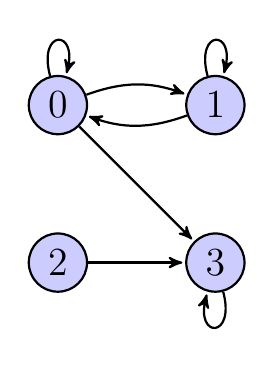
\begin{tikzpicture}[->,>=stealth',shorten >=1pt,auto,node distance=2cm,
 			thick,main node/.style={circle,fill=blue!20,draw,
 				font=\sffamily\Large\bfseries,minimum size=5mm}]
 			
 			\node[main node] (A) {$0$};
 			\node[main node] (B) [right of=A] {$1$};
 			\node[main node] (C) [below of=A] {$2$};
 			\node[main node] (D) [below of=B] {$3$};
 			
 			\path[every node/.style={font=\sffamily\small,
 				fill=white,inner sep=1pt}]
 			(A) edge [loop above] (A)
 			(A) edge [bend left=20] (B)
 			(A)edge (D)
 			(B) edge [loop above] (B)
 			(B) edge [bend left=20] (A)
 			(C) edge (D)
 			(D) edge [loop below] (D);
 		\end{tikzpicture}
 	\end{center}
 	
 	$R_1$ is not reflexive as every vertex doesn't include an edge loop (an arrow that goes from the vertex to the itself). Neither is it symmetric as not all vertices is connected by arrows that goes to and from another arrow. And last, the graph doesn't satisfy the property of transivity, as not all vertices are connected.\\
 	\pagebreak
 	
 	$R_2$ has the following graph:
 	
 	\begin{center}
 		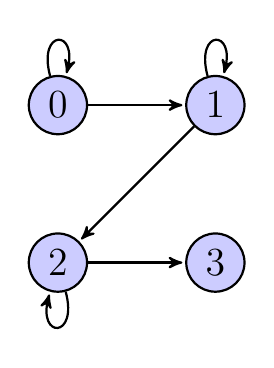
\begin{tikzpicture}[->,>=stealth',shorten >=1pt,auto,node distance=2cm,
 			thick,main node/.style={circle,fill=blue!20,draw,
 				font=\sffamily\Large\bfseries,minimum size=5mm}]
 			
 			\node[main node] (A) {$0$};
 			\node[main node] (B) [right of=A] {$1$};
 			\node[main node] (C) [below of=A] {$2$};
 			\node[main node] (D) [below of=B] {$3$};
 			
 			\path[every node/.style={font=\sffamily\small,
 				fill=white,inner sep=1pt}]
 			(A) edge [loop above] (A)
 			(A) edge (B)
 			(B) edge [loop above] (B)
 			(C) edge [loop below] (C)
 			(B) edge (C)
 			(C) edge (D);
 		\end{tikzpicture}
 	\end{center}
 	
 	This relation doesn't satisfy any properties as not all vertices have an edge loop, and all the vertices are connected in one direction only, and last there is a distinct path from $0$ to $3$.\\
 	
 	Let's look at the graph of $R_3$:
 	
 	\begin{center}
 		\begin{tikzpicture}[->,>=stealth',shorten >=1pt,auto,node distance=2cm,
 			thick,main node/.style={circle,fill=blue!20,draw,
 				font=\sffamily\Large\bfseries,minimum size=5mm}]
 			
 			\node[main node] (B) [left of=C] {$1$};
 			\node[main node] (C) [right of=B] {$2$};
 			
 			\path[every node/.style={font=\sffamily\small,
 				fill=white,inner sep=1pt}]
 			(B) edge [bend left=20] (C)
 			(C) edge [bend left=20] (B);
 		\end{tikzpicture}
 	\end{center}
 	
 	This relation however seems to satisfy the reflexive property as every vertex has an edge loop. Furthermore it must also be symmetric as every vertex is connected to another vertex by two arrows going out and in. And last, it also seems to be an transitive relation.\\
 	
 	The graph of $R_4$:
 	
 	\begin{center}
 		\begin{tikzpicture}[->,>=stealth',shorten >=1pt,auto,node distance=2cm,
 			thick,main node/.style={circle,fill=blue!20,draw,
 				font=\sffamily\Large\bfseries,minimum size=5mm}]
 			
 			\node[main node] (A) [left of =B] {$1$};
 			\node[main node] (B) [right of =A] {$2$};
 			\node [main node] (C)  [below of=A] {$3$};
 			\path[every node/.style={font=\sffamily\small,
 				fill=white,inner sep=1pt}]
 			(A) edge [bend left=20] (B)
 			(B) edge [bend left=20] (A)
 			(A) edge [bend left=20] (C)
 			(C) edge [bend left=20] (A);
 			
 		\end{tikzpicture}
 	\end{center}
 	
 	$R_4$ doesn't seem to satisfy any property as no vertex has a loop edge, neither is all connected, and last; no triangle connection is present as by definition of transivity.\\
 	\pagebreak
 	
 	The graph of $R_5$:
 	
 	\begin{center}
 		\begin{tikzpicture}[->,>=stealth',shorten >=1pt,auto,node distance=2cm,
 			thick,main node/.style={circle,fill=blue!20,draw,
 				font=\sffamily\Large\bfseries,minimum size=5mm}]
 			
 			\node[main node] (A) [left of =B] {$0$};
 			\node[main node] (B) [right of =A] {$1$};
 			\node [main node] (C)  [below of=A] {$2$};
 			\path[every node/.style={font=\sffamily\small,
 				fill=white,inner sep=1pt}]
 			(A) edge [loop above] (A)
 			(A) edge (B)
 			(A) edge (C)
 			(B) edge (C);
 		\end{tikzpicture}
 	\end{center}
 
 	$R_5$ is neither reflexive or symmetric as only one vertex contains an edge loop, and while all vertices might be connected, they are not connected bidirectional. But $R_5$ is transitive as all vertices are connected.\\
 	
 	The graph of $R_6$:
 	
 	\begin{center}
 		\begin{tikzpicture}[->,>=stealth',shorten >=1pt,auto,node distance=2cm,
 			thick,main node/.style={circle,fill=blue!20,draw,
 				font=\sffamily\Large\bfseries,minimum size=5mm}]
 			
 			\node[main node] (A) [left of =B] {$0$};
 			\node[main node] (B) [right of =A] {$1$};
 			\node [main node] (C)  [below of=A] {$2$};
 			\path[every node/.style={font=\sffamily\small,
 				fill=white,inner sep=1pt}]
 			(A) edge (B)
 			(A) edge (C);
 		\end{tikzpicture}
 	\end{center}
 
 	$R_6$ has no properties as none of them are satisfies. We'll make it short for now.
 	
 	The graph of $R_7$:
 	
 	\begin{center}
 		\begin{tikzpicture}[->,>=stealth',shorten >=1pt,auto,node distance=2cm,
 			thick,main node/.style={circle,fill=blue!20,draw,
 				font=\sffamily\Large\bfseries,minimum size=5mm}]
 			
 			\node[main node] (A) [above left of =C] {$0$};
 			\node[main node] (B) [above right of =C] {$2$};
 			\node [main node] (C)  [below left of=B] {$3$};
 			\path[every node/.style={font=\sffamily\small,
 				fill=white,inner sep=1pt}]
 			(A) edge (C)
 			(B) edge (C);
 		\end{tikzpicture}
 	\end{center}
 	
 	Again, no properties satisfied.\\
 	
 	Let's take a look on the last relation $R_8$:
 	
 	\begin{center}
 		\begin{tikzpicture}[->,>=stealth',shorten >=1pt,auto,node distance=2cm,
 			thick,main node/.style={circle,fill=blue!20,draw,
 				font=\sffamily\Large\bfseries,minimum size=5mm}]
 			
 			\node[main node] (A) [left of =B] {$0$};
 			\node[main node] (B) [right of =A] {$1$};
 			\path[every node/.style={font=\sffamily\small,
 				fill=white,inner sep=1pt}]
 			(A) edge [loop above] (A)
 			(B) edge [loop above] (B);
 		\end{tikzpicture}
 	
 	\end{center}
 
 No properties satisfied.
\end{document}

 